\chapter{Application Resto}
L'\ar est une application destinée au grand public de consultation de restaurant à distance et de livraison de restaurant.

Les utilisations courantes de l'application sont : 
\begin{itemize}
	\item dans un restaurant comme cartes virtuelles en remplacement des cartes physiques ;
	\item réservation d'une table dans un restaurant ;
	\item commande depuis un autre lieu que le restaurant pour la livraison.
\end{itemize}

Pour trouver un restaurant sur l'application, l'utilisateur doit se géolocaliser et ensuite choisir le restaurant soit par les restaurants à proximité soit par les favoris soit par recherche via un moteur de recherche.

Un restaurant est organisé de la manière suivante : Un restaurant possède des cartes de plusieurs types et chaque carte peut avoir trois usages. Une carte peut contenir une carte ou un article. Un article peut être un plat ou une boisson.

Les trois usages d'une carte sont : 
\begin{itemize}
	\item en tant que carte de haut niveau : \\
	Une carte de haut niveau contient d'autres cartes et des articles
	\item en tant que carte d'accueil: \\
	Une carte d'accueil est celle qui sera affichée par défaut à l'utilisateur.
	\item en tant que carte autres:\\
	Une carte autre est une carte simple. 
\end{itemize}

Dans la suite de ce chapitre il sera présenté les différents composants de l'application en détaillant les diagrammes et en présentant les travaux réalisés.

\section{Contexte du système}
Dans cette section il est présenté le diagramme de contexte du système afin de le localiser dans son environnement, les acteurs qui interagissent  avec le système.
\begin{figure}[H]
	\centering
	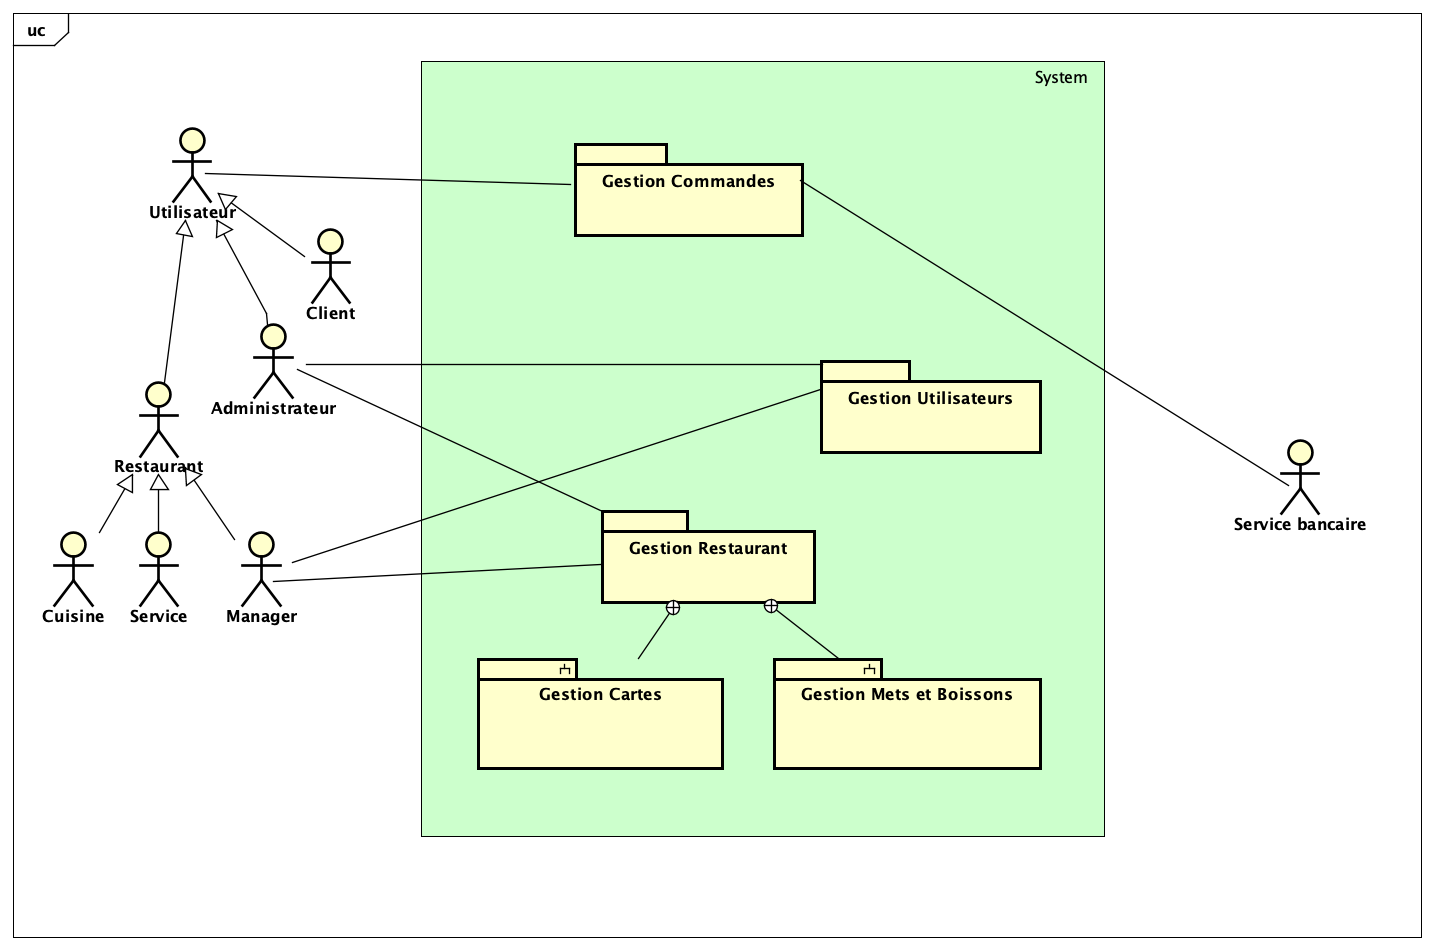
\includegraphics[scale=0.4]{assets/images/Restaurant_system.png}
	\caption{Diagramme de contexte de l'\ar}
	\label{fig.9}
\end{figure}
L'\ut est l'acteur principal. Il a plusieurs profil non cumulable. Comme indiqué sur la figure \ref{fig.9} les différents profil sont : le manager, le service, la cuisine, l'administrateur et le client. 

Un \ut c'est-à-dire tous les profils peut gérer une commande. Un administrateur peut gérer les utilisateurs et les restaurants.

Un manager peut aussi gérer un restaurant et un seul.

L'acteur secondaire du système est la banque ou le service bancaire. Son rôle est de valider les paiements.

\section{Caractéristique de l'utilisateur}
L'application est destinée à l'utilisation du grand public et des restaurants. Elle ne requiert aucune compétence particulière à part le fait de savoir utiliser un smartphone.

\section{Contraintes principaux de développement}
L'application a été développé pour la plateforme mobile iOS et selon le paradigme orienté objet. L'application étant assez complexe, il est important de la concevoir selon une architecture logicielle pour rendre facile son utilisation.

\section{Besoins fonctionnels}
Il s'agit ici de décrire les besoins fonctionnels du système à travers les cas d'utilisation de l'application. Pour une meilleure étude des fonctionnalités de l'application, j'ai décomposé l'application par paquet. Nous allons donc étudié les différents paquets.
\subsection{Paquet gestion des cartes}
\begin{figure}[H]
	\centering
	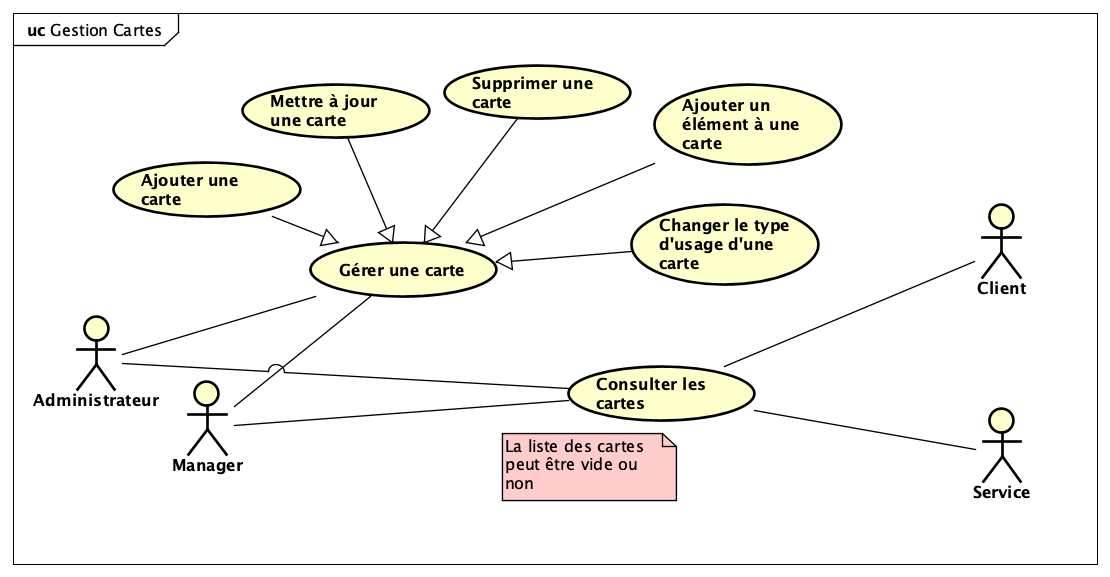
\includegraphics[scale=0.4]{assets/images/gestion_cartes_uc.png}
	\caption{Diagramme de cas d'utilisation de la gestion des cartes}
	\label{fig.10}
\end{figure}
Le diagramme sur la figure \ref{fig.10}, présente une vue générale des cas d'utilisation du paquet. Chaque cas d'utilisation est lié à un acteur et décrit un état du système. Dans les prochaines sections, il sera détaillé les cas d'utilisation par acteur.
\subsubsection{Description des cas d'utilisation par acteur}
Le système est composé de quatre acteurs principaux qui sont : l'\adm, le \m, le \sev, et le \cl. Pour comprendre le rôle joué par chacun, nous procédons ici à une brève description de chacun d'eux.
\subsubsection*{L'\adm}
L'\adm,  peut ajouter une carte, mettre à jour les informations d'une carte, supprimer une carte et ajouter un article à une carte. Il peut aussi consulter les cartes. L'\adm peut effectuer ces actions sur les cartes de tous les restaurants.

\subsubsection*{Le \m}
Il peut effectuer les mêmes actions que l'\adm mais ces actions sont limitées aux cartes du restaurant qu'il gère.

\subsubsection*{Le \sev}
Il ne peut que consulter les cartes du restaurant dans lequel il est associé et voir leurs contenus.

\subsubsection*{Le \cl}
Il peut consulter les cartes de tous les restaurants dans son lieu de résidence et voir leurs contenus.

\subsubsection{Spécification des structures de données}
\begin{figure}[H]
	\centering
	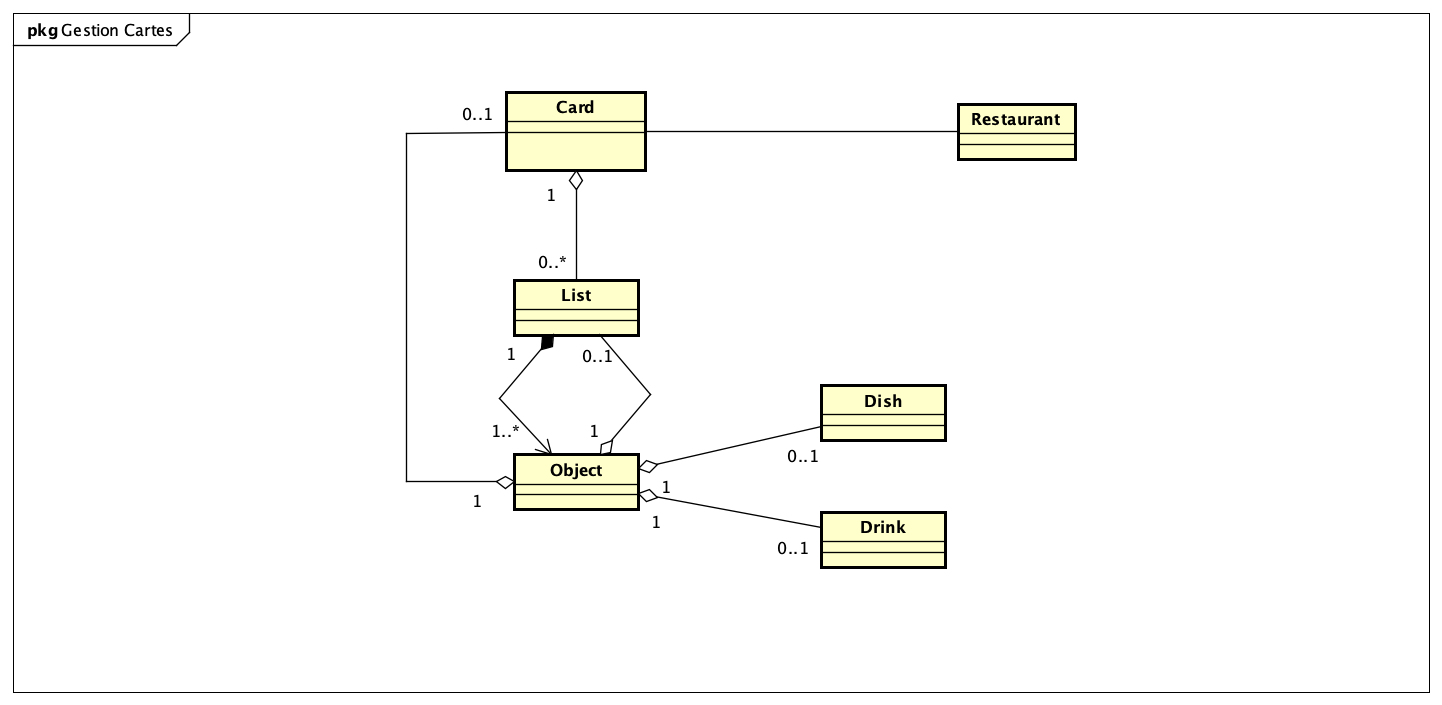
\includegraphics[scale=0.4]{assets/images/gestion_card_cd.png}
	\caption{Diagramme de classe de la gestion des cartes}
	\label{fig.11}
\end{figure}

Comme décrit sur le diagramme de la figure \ref{fig.11}, un restaurant dispose de plusieurs cartes. Une carte possède zero ou plusieurs listes. Une liste peut exister sans carte. Une liste est composée de un ou plusieurs objet qui est soit un plat ou une boisson. Un objet peut posséder aussi une liste ou une carte.

\subsection{Paquet gestion d'un article}
Le diagramme de la figure \ref{fig.12} présente une vue générale des cas d'utilisations du paquet. Chaque cas d'utilisation est lié à un acteur et décrit un état du système.
\begin{figure}[H]
	\centering
	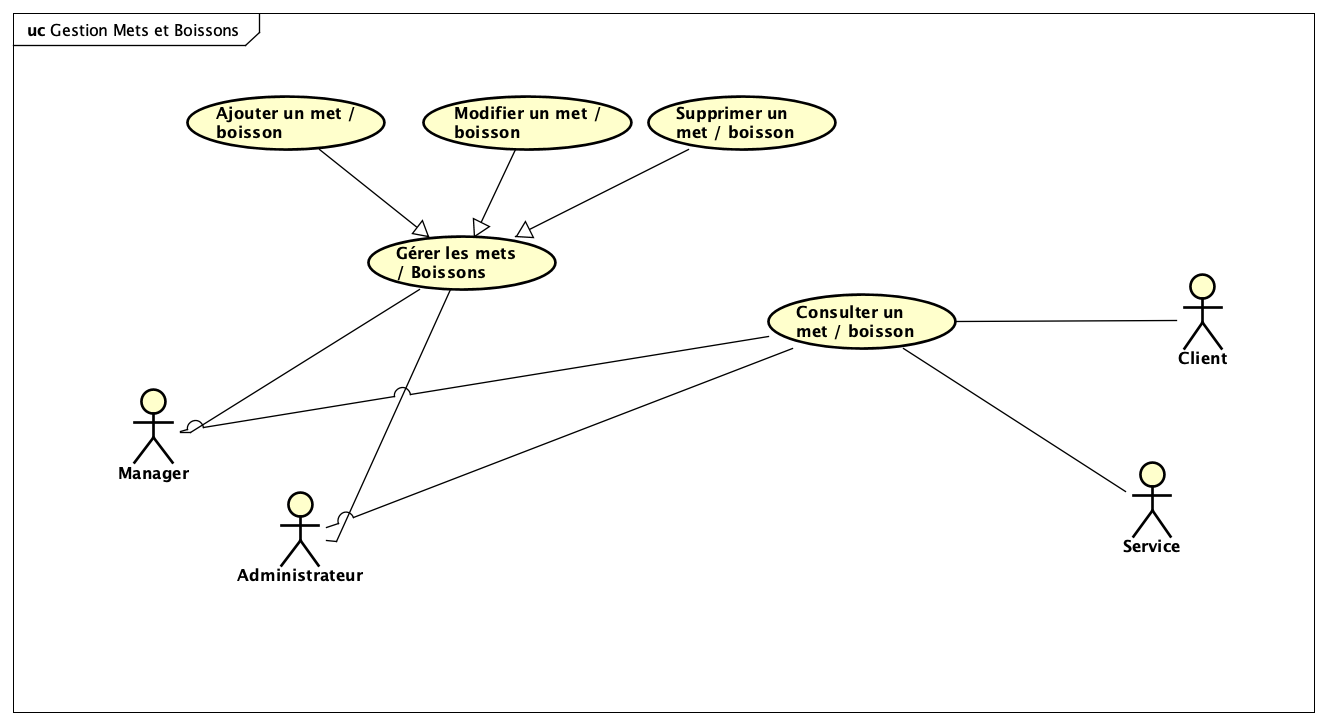
\includegraphics[scale=0.4]{assets/images/gestion_items_uc.png}
	\caption{Diagramme de cas d'utilisation de la gestion d'un article}
	\label{fig.12}
\end{figure}
\subsubsection{Description des cas d'utilisation par acteur}
Les acteurs intervenant dans ce paquet sont les mêmes que le paquet précédent.
\subsubsection*{L'\adm}
Il peut ajouter, modifier les informations et supprimer un plat ou une boisson de tous les restaurants. Il peut aussi consulter les articles des restaurants.

\subsubsection*{Le \m}
Il peut ajouter, modifier, supprimer et consulter un plat ou une boisson de son restaurant.

\subsubsection*{Le \sev}
Il peut consulter les articles du restaurant auquel il est associé.

\subsubsection*{Le \cl}
Il peut consulter les articles de tous les restaurants dans son lieu de résidence.

\subsubsection{Spécification des structures de données}
\begin{figure}[H]
	\centering
	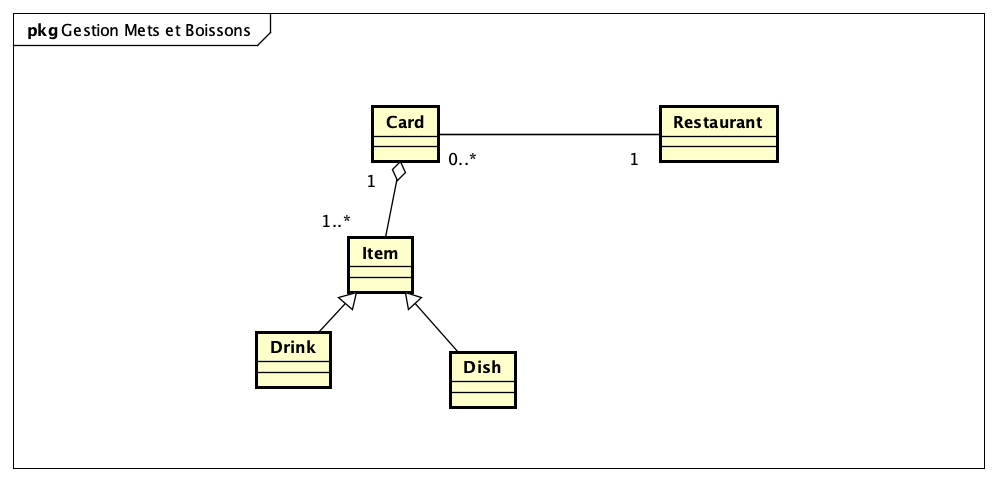
\includegraphics[scale=0.4]{assets/images/gestion_items.png}
	\caption{Diagramme de classe de la gestion d'un article}
	\label{fig.13}
\end{figure}

D'après le diagramme de la figure \ref{fig.13}, un article est soit un plat soit une boisson et il appartient à une carte.

\subsection{Paquet gestion des commandes}
Le diagramme de la figure  \ref{fig.14} présente une vue générale des cas d'utilisation du paquet. Chaque cas d'utilisation est lié à un acteur et décrit un état du système.
\begin{figure}[H]
	\centering
	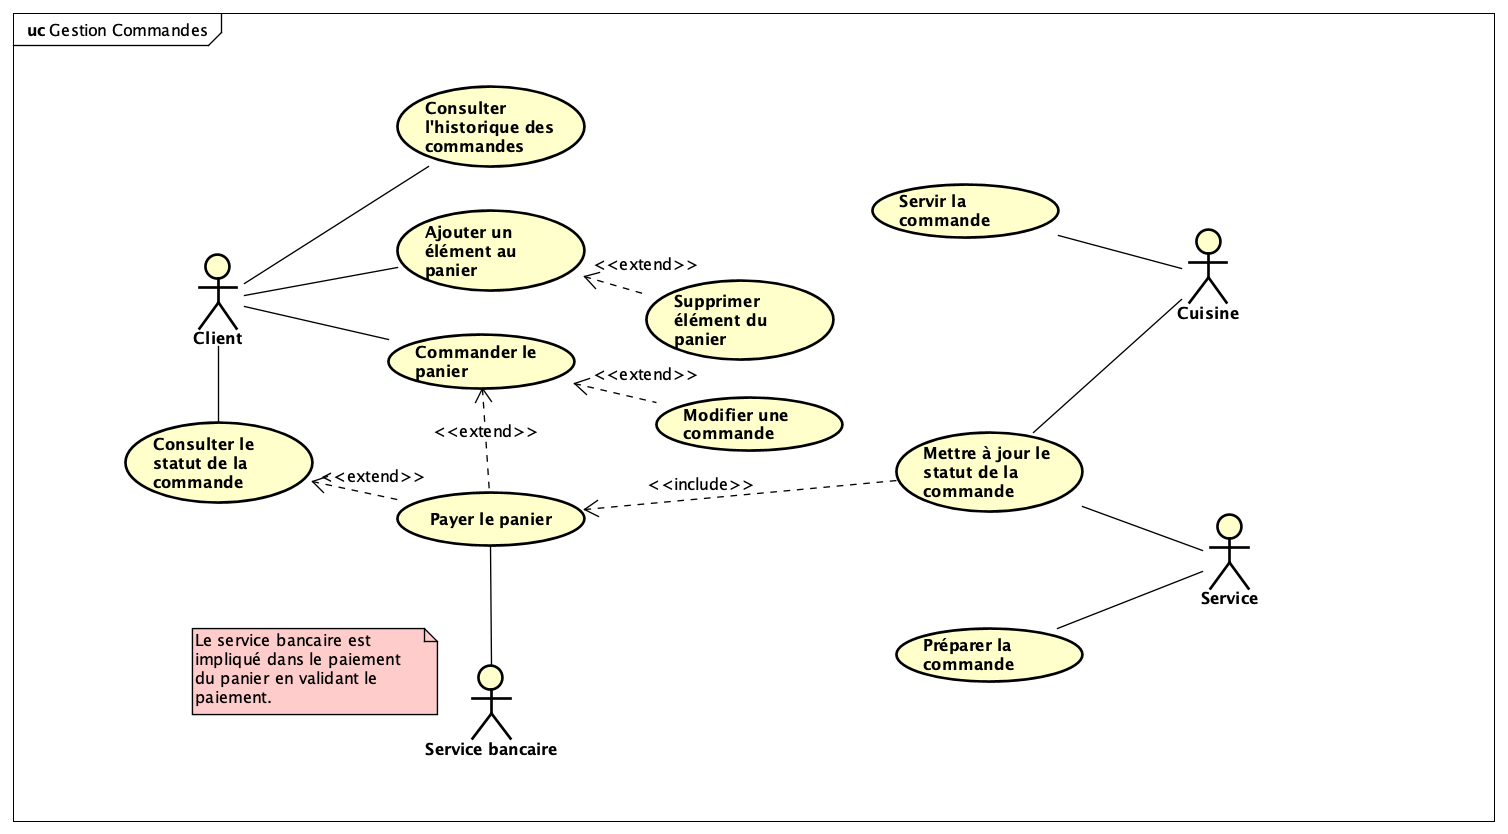
\includegraphics[scale=0.4]{assets/images/gestion_command_uc.png}
	\caption{Diagramme de cas d'utilisation de la gestion des commandes}
	\label{fig.14}
\end{figure}
\subsubsection{Description des cas d'utilisation par acteur}
Les principaux acteurs intervenant dans le fonctionnement de ce paquet sont : le \cl, le \emph{service bancaire}, le \sev, et la \csn.
\subsubsection*{Le \cl}
Il peut ajouter un article au panier, commander et payer le panier, consulter le statut d'une commande, consulter l'historique des commandes, modifier une commande ou encore supprimer un article du panier.

\subsubsection*{Le \emph{service bancaire}}
Son rôle est de valider le paiement d'une commande.

\subsubsection*{Le \sev}
Il peut mettre à jour le statut d'une commande et servir une commande.

\subsubsection*{La \csn}
Elle peut préparer une commande et mettre à jour le statut d'une commande.

\subsubsection{Spécification des structures de données}
\begin{figure}[H]
	\centering
	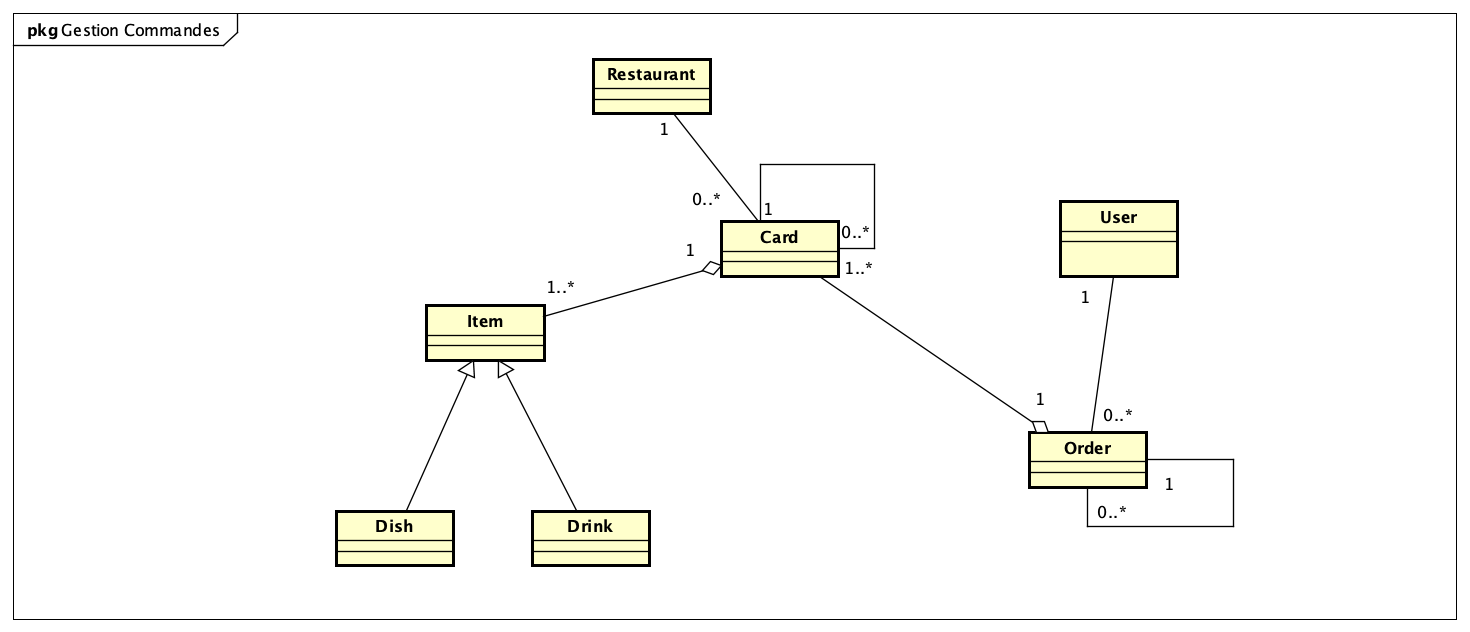
\includegraphics[scale=0.4]{assets/images/gestion_command_cd.png}
	\caption{Diagramme de classe de la gestion des commandes}
	\label{fig.15}
\end{figure}

D'après le diagramme de la figure \ref{fig.15}, une commande contient un ou plusieurs cartes. Elle peut être liée à une autre commande pour constituer une commande de groupe.

D'une manière spécifique, une commande étant lié à un restaurant, le concept de panier aussi est lié d'un couplage fort au restaurant. Ainsi si pour une raison, le \cl sort du restaurant courant dans le cas où il a des commandes non validées, et visite un autre restaurant, le panier courant sera celui du nouveau restaurant et donc vide.

\subsection{Description générale}
Comme défini sur la figure \ref{fig.9}, l'application est composée de paquets et chaque paquet communique avec l'autre. L'architecture globale de l'application est une architecture client-serveur. Le serveur communique avec le client via une API REST dont le module de sécurité est le token de session lié automatiquement à un utilisateur.

\section{Spécification des interfaces externes}
\subsection{Interface Matériel/logiciel}
\subsubsection*{Configuration minimale sur laquelle le système peut s'exécuter}
Pour faire fonctionner l'application sur un appareil mobile, l'appareil devra avoir les configurations minimales suivantes :
\begin{itemize}
	\item Matériel : Tous les smartphones iOS supportant les configurations minimales au niveau logiciel.
	\item Logiciel : Tous les smartphones  iOS supportant au moins la version 13.0 de l'OS.
\end{itemize}

\subsubsection*{Protocole d'échange}
Pour le fonctionnement du système les protocoles utilisés sont le REST qui est basé sur les verbes HTTP.

\subsection{Interface logiciel/logiciel}
Pour développer l'application, les outils suivants ont été utilisés:
\begin{itemize}
	\item lanagages et bibliothèques de développement 
	\begin{itemize}
		\item[-] Swift 5.1
		\item[-] Objective C 2.0
		\item[-] Cocoa Touch Framework 
	\end{itemize}
	\item Outils de développement
	\begin{itemize}
		\item[-] XCode 11.0
		\item[-] Git 2.2
		\item[-] GitLab
		\item[-] Mac Mini 2019 et MacOS Catalina
		\item[-] Simulateur iPhone 11 Pro Max
	\end{itemize}
\end{itemize}

\subsection{Interface homme-machine}
\subsubsection*{Structure}
\begin{figure}[H]
	\centering
	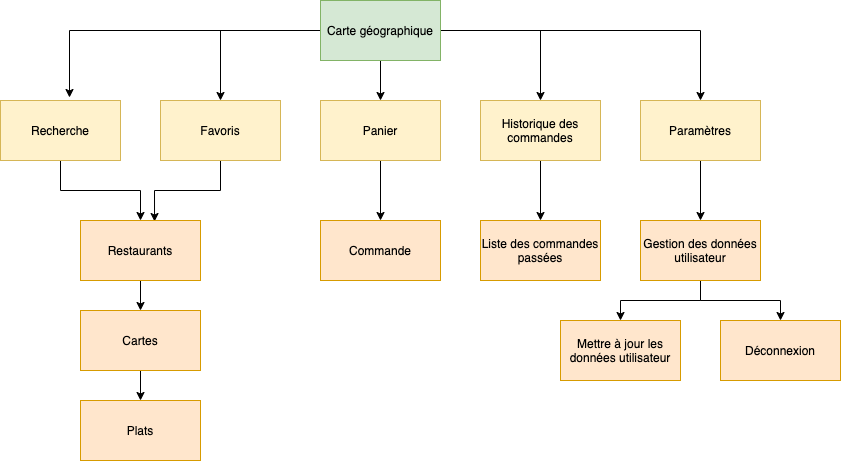
\includegraphics[scale=0.5]{assets/images/ihm_structure.png}
	\caption{Structure \gls{IHM} de l'application client}
	\label{fig.16}
\end{figure}
Il est décrit sur la figure \ref{fig.16}, la structure générale de l'\gls{IHM} de l'application client. Le point d'entrée de l'application est la carte géographique. De cette carte, l'utilisateur peut se géolocaliser afin de réduire la zone de recherche des restaurants. En réalité il existe deux points d'entrée pour l'application qui sont liées à deux scénarios. Le cas ou c'est un nouveau utilisateur ou un habitué. Si l'utilisateur est un nouveau, son point d'entrée est la carte mais s'il est un habitué son point d'entrée est l'onglet des favoris. 

Le contenu des recherches et des favoris contient des restaurants. D'un restaurant, l'utilisateur peut consulter les cartes, les plats et effectuer une commande.

Le panier est l'onglet dans lequel l'utilisateur peut voir sa commande courante.

Une fois la commande passée, l'utilisateur peut consulter l'historique des commandes.

L'utilisateur peut gérer ses informations personnelles depuis l'onglet Paramètres ou se déconnecter.

\begin{figure}[H]
	\centering
	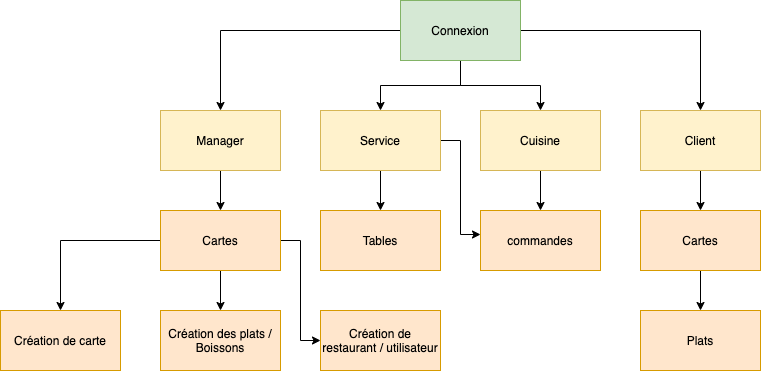
\includegraphics[scale=0.5]{assets/images/pro_ihm.png}
	\caption{Structure \gls{IHM} de l'application pro}
	\label{fig.17}
\end{figure}
Il est décrit sur le diagramme de la figure \ref{fig.17}, la structure générale de l'\gls{IHM} de l'application pro. Le point d'entrée de l'application est la page de connexion. L'utilisateur connecté possède un profil. Selon son profil, l'utilisateur peut effectuer certaines actions.

Ainsi le \m pourra créer des cartes des plats ou encore un restaurant ou un utilisateur.

Le service peut voir l'organisation des tables et consulter les commandes.

La cuisine peut voir uniquement les commandes.

Le client peut consulter les cartes du restaurants et passer une commande.

Pour des raisons de sécurité, pour changer de profil, l'utilisateur est forcément rediriger vers un écran d'authentification.
\section{Déroulement du stage}
\subsection{Développement et difficultés rencontrés}
L'\ar est composée de deux modules. Le module client et le module pro. Les deux modules ont été développés en deux applications différentes. Pour rendre l'application évolutive et pour éviter un couplage fort entre les composants, j'ai adopté une des méthodes de Clean architecture\cite{clean_arch} développé par \textbf{Robert C. Martin\cite{clean_code}} appliqué au développement iOS au cours du développement. Cet architecture est nommé \textbf{\gls{VIPER}\cite{viper}}.
\begin{figure}[H]
	\centering
	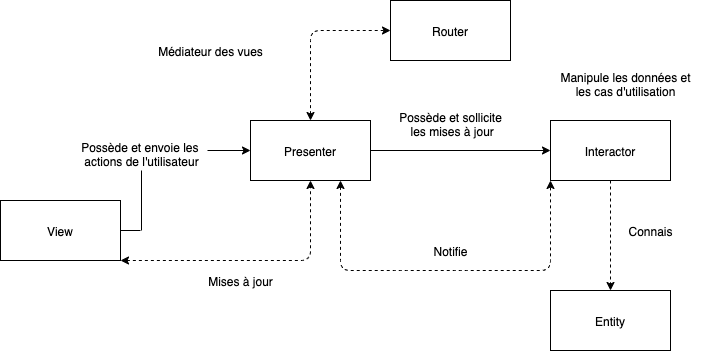
\includegraphics[scale=0.5]{assets/images/viper_communication_details.png}
	\caption{Architecture \gls{VIPER}}
	\label{fig.18}
\end{figure}

Chaque entité sur le diagramme, représente une classe au sens orienté objet. Ainsi la classe View est celle décrivant la vue. La classe Presenter met à jour la vue et demande à la classe Router de changer de vue si nécessaire ou à la classe Interactor de lui fournir les données nécessaires.

Comme décrit ci-haut on constate que chaque a une seule responsabilité ce qui respecte le fondement même des programmes orienté objet.

L'objectif de cet architecture est de permettre une évolutivité totale du code, une testabilité facile et un couplage très faible.

Appliqué à tous les composants de l'application, cette architecture m'a permis de la réutilisation des composants sans modifier le code. L'écriture des tests unitaires a été facile.

Un exemple de diagramme de classe d'un composant utilisant cette architecture est disponible dans l'annexe.

Les difficultés que j'ai rencontré au cours du développement résident lors de l'ajout d'un article au panier. Chaque article étant lié à une carte, c'était compliqué de réaliser la fonctionnalité d'ajout  d'article au panier. Finalement j'ai résolu le problème en créant une classe générique fictive de navigation entre les cartes et j'ai adopté le pattern Observer pour gérer le panier.

\begin{figure}[H]
	\centering
	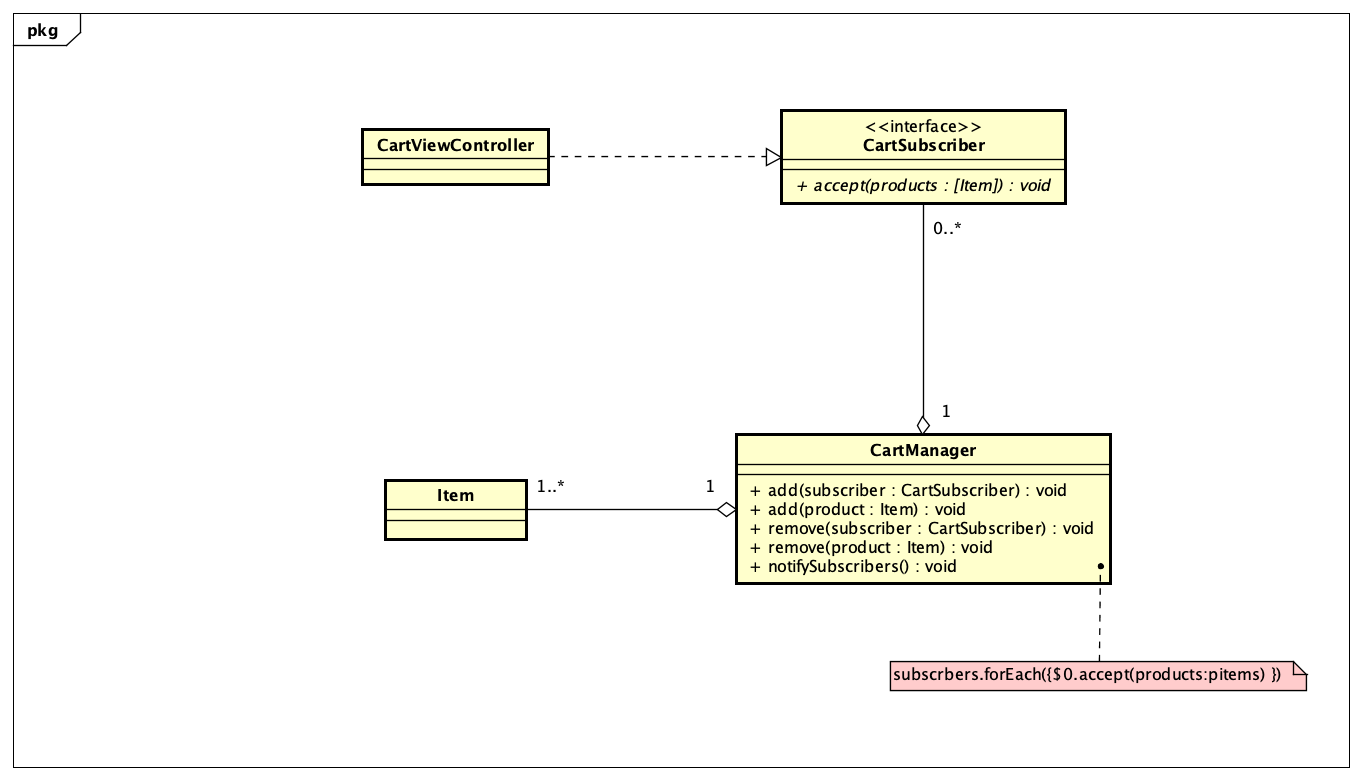
\includegraphics[scale=0.3]{assets/images/cart_management.png}
	\caption{Pattern Observer décrivant la gestion du panier}
	\label{fig.19}
\end{figure}

\section{Planning daté du travail}
Le diagramme de Gantt de la figure \ref{fig.20} présente ma charge de travail sur le développement de l'\ar
\begin{figure}[H]
	\centering
	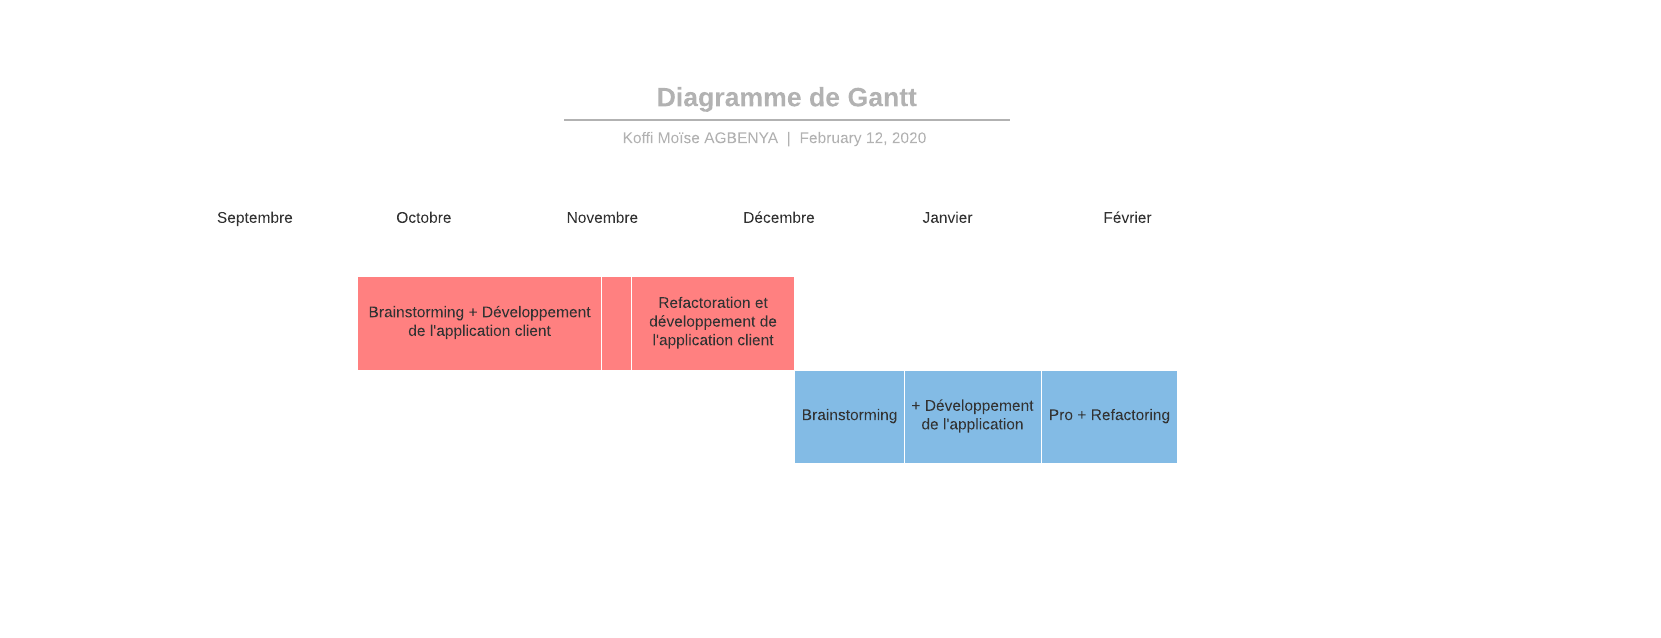
\includegraphics[scale=0.8]{assets/images/Gantt_resto.png}
	\caption{Diagramme de Gantt du projet Resto}
	\label{fig.20}
\end{figure}

\subsection{Conditions de travail}
\subsubsection*{Horaires}
Mes horaires de travail pendant le stage étaient de 08h à 17h avec une pause de 1h soit entre 12h et 13h ou 13h et 14h. L'horaire journalier de travail est de 8h au Luxembourg.

\subsubsection*{Badges et Accès}
L'accès aux bureaux requiert un badge. J'ai obtenu mon badge dès le début de mon stage.

\subsubsection*{Accès internet}
L'accès à internet n'est pas restreint dans l'entreprise mais l'entreprise dispose d'un proxy pour tout échange avec l'extérieur.